\documentclass[epsfig,10pt,fullpage]{article}

\newcommand{\LabNum}{5}
\newcommand{\CommonDocsPath}{../../common/docs}
\addtolength{\textwidth}{1.5in}
\addtolength{\oddsidemargin}{-0.75in}
\addtolength{\topmargin}{-0.75in}
\addtolength{\textheight}{1.5in}
\addtolength{\evensidemargin}{0.75in}
\setlength\parindent{0pt}
\raggedbottom

\usepackage{ae,aecompl}
\usepackage{epsfig,float,times}
\usepackage[hypcap]{caption}
\usepackage[pdftex, colorlinks]{hyperref}
\usepackage{graphicx}
\usepackage[usenames, dvipsnames]{color}
\usepackage{rotating}
\usepackage{tikz}
\usetikzlibrary{automata,positioning}
\usepackage{placeins}

\widowpenalty 10000
\clubpenalty 10000

\newcommand{\red}[1]{{\color{red}\sf{#1}}}
\newcommand{\green}[1]{{\color{green}\sf{#1}}}
\newcommand{\blue}[1]{{\color{blue}\sf{#1}}}
\definecolor{PineGreen}{rgb}{0.0, 0.47, 0.44}
\definecolor{ForestGreen}{rgb}{0.13, 0.55, 0.13}
\definecolor{Brown}{rgb}{0.59, 0.29, 0.0}

\newcommand{\UPDatePublished}{Oct 2021}
\newcommand{\versnum}{21.1} %version number quartus/AMP
\newcommand{\quartusname}{Quartus\textsuperscript{\textregistered} Prime}	
\newcommand{\UPTextBar}{For \quartusname{} \versnum{}}
\newcommand{\thisyear}{2021 } %for copyright
\newcommand{\company}{FPGAcademy.org}
\newcommand{\longteamname}{FPGAcademy.org}
\newcommand{\teamname}{FPGAcademy}
\newcommand{\website}{FPGAcademy.org}

\newcommand{\productAcronym}{AMP}
\newcommand{\productNameShort}{Monitor Program}

\newcommand{\productNameMedTM}{A Monitor Program}
\newcommand{\productNameMed}{A Monitor Program}

%\newcommand{\headerLogoFilePath}[1]{#1/FPGAcademy.png}

% listings is a package that supports encapsulating source code in LaTeX conveniently
\usepackage{listings}

\def\expandparam\lstinputlisting[#1]#2{\edef\tmp{\noexpand\lstinputlisting[#1]{#2}}\tmp}

%%%%%%%%%%%%%%%%%%%% Source Code Formatting %%%%%%%%%%%%%%%%%%%%
\definecolor{globalCommentColour}{rgb}{0.588,0.588,0.588}

%%%%%%%%%%%%%%%%%%%%%%%%%%%%%%%%%%%%%%%%%%%%%%%%%%%%
% Defining language style
% NiosII ASM
\lstdefinelanguage[NiosII]{Assembler} {
  morekeywords={add, addi, and, andhi, andi, beq, bge, bgeu, bgt, bgtu, ble,  bleu, blt, bltu, bne, br, break,
  bret, call, callr, cmpeq, cmpeqi, cmpge, cmpgei, cmpgeu, cmpgeui, cmpgt, cmpgti, cmpgtu, cmpgtui, cmple,
  cmplei, cmpleu, cmpleui, cmplt, cmplti, cmpltu, cmpltui, cmpne, cmpnei, custom, div, divu, eret, flushd,
  flushda, flushi, flushp, initd, initda, initi, jmp, jmpi, ldb, ldbio, ldbu, ldbuio, ldh, ldhio, ldhu, ldhuio,
  ldw, ldwio, mov, movhi, movi, movia, movui, mul, muli, mulxss, mulxsu, mulxuu, nextpc, nop, nor, or, orhi, ori,
  rdctl, rdprs, ret, rol, roli, ror, sll, slli, sra, srai, srl, srli, stb, stbio, sth, sthio, stw, stwio,
  sub, subi, sync, trap, wrctl, wrtcl, wrprs, xor, xori, xorhi, xori},
  morekeywords=[2]{.abort, .ABORT, .align, .app-file, .ascii, .asciz, .balign, .byte, .comm, .data, .def,
  .desc, .dim, .double, .eject, .else, .end, .endef, .endif, .equ, .equiv, .err, .extern, .file, .fill, .float,
  .global, .globl, .hword, .ident, .if, .include, .int, .irp, .irpc, .lcomm, .lflags, .line, .linkonce, .ln,
  .list, .long, .macro, .mri, .nolist, .octa, .org, .p2align, .psize, .quad, .rept, .sbttl, .scl, .section,
  .set, .short, .single, .size, .sleb128, .skip, .space, .stadb, .stabn, .stabs, .string, .symver, .tag,
  .text, .title, .type, .val, .uleb128, .word},
  morekeywords=[3]{et, bt, gp, sp, fp, ea, sstatus, ra, pc, status, estatus, bstatus, ienable, ipending, cpuid,
  exception, pteaddr, tlbacc, tlbmisc, eccinj, badaddr, config, mpubase, mpuacc},
  sensitive=t,
  alsoletter=.,
  morestring=[b]",
  morecomment=[s]{/*}{*/},
  morecomment=[l]\#,
}[keywords,comments,strings]
   
%% NOTE: morekeywords=[2] are GNU directives.
   
\definecolor{niosInstructionColour}{rgb}{0.000,0.608,0.000}
\definecolor{niosDirectiveColour}{rgb}{0.000,0.000,0.902}
\definecolor{niosSpecialRegColour}{rgb}{0.000,0.000,0.000}
\definecolor{niosStringColour}{rgb}{0.808,0.482,0.000}
   
%% NOTE: To make bold use: =\bfseries\color{<colour>}
\lstdefinestyle{defaultNiosStyle} {
  language=[NiosII]{Assembler},
  stringstyle=\color{niosStringColour},
  keywordstyle=\color{niosInstructionColour},
  keywordstyle=[2]\color{niosDirectiveColour},
  keywordstyle=[3]\itshape\color{niosSpecialRegColour}
}
%%%%%%%%%%%%%%%%%%%%%%%%%%%%%%%%%%%%%%%%%%%%%%%%%%%%

%%%%%%%%%%%%%%%%%%%%%%%%%%%%%%%%%%%%%%%%%%%%%%%%%%%%
% Defining language style
% ArmA9 ASM
\lstdefinelanguage[ArmA9]{Assembler} {
  morekeywords={ADC, ADD, ADDS, AND, ANDS, B, BAL, BEQ, BGE, BGT, BL, BLT, BIC, BKPT, BLX, BNE, BX, CDP, CLZ, CMN, CMP, EOR,
  EORS, LDC, LDM, LDR, LDRB, LDRBT, LDRH, LDRSB, LDRSH, LDRT, LSL, MCR, MLA, MOV, MOVW, MOVT, MRC, MRS, MSR, MUL, MVN, ORR, PLD,
  ROR, RSB, RSC, SBC, SMLAL, SMULL, STC, STM, STR, STRB, STRBT, STRH, STRT, SUB, SUBS, SWI, SWP, SWPB, TEQ, UMLAL,
  PUSH, POP, MOVS, RORS, LSR},
  morekeywords=[2]{.abort, .ABORT, .align, .app-file, .ascii, .asciz, .balign, .byte, .comm, .data, .def,
  .desc, .dim, .double, .eject, .else, .end, .endef, .endif, .equ, .equiv, .err, .extern, .file, .fill, .float,
  .global, .globl, .hword, .ident, .if, .include, .int, .irp, .irpc, .lcomm, .lflags, .line, .linkonce, .ln,
  .list, .long, .macro, .mri, .nolist, .octa, .org, .p2align, .psize, .quad, .rept, .sbttl, .scl, .section,
  .set, .short, .single, .size, .sleb128, .skip, .space, .stadb, .stabn, .stabs, .string, .symver, .tag,
  .text, .title, .type, .val, .vectors, .uleb128, .word},
  morekeywords=[3]{SP, PC, MIDR, CTR, TCMTR, TLBTR, MPIDR, ID_PFR0, ID_PFR1, ID_DFR0, ID_MMFR0, ID_MMFR1, ID_MMFR2,
  ID_MMFR3, ID_ISAR0, ID_ISAR1, ID_ISAR2, ID_ISAR3, ID_ISAR4, CCSIDR, CLIDR, AIDR, CSSELR, TTBR0, TTRB1, TTBR2, DACR,
  DFSR, IFSR, ADFSR, AIFSR, DFAAR, IFAR, ICIALLUIS, BPIALLIS, PAR, ICIALLU, ICIMVAU, BPIALL, DCIMVAC, DCISW, V2PCWPR,
  DCCVAC, DCCSW, DDIMVAC, DCISW, TLBALLIS, TLBIMVAIS, TLBIASIDIS, TLBIMVAAIS, TLBIALL, TLBIMVA, TLBIASID, TLBIMVAA,
  PMCR, PMCNTENSET, PMCNTENCLR, PMOVSR, PMSWINC, PMSELR, PMXEVTYPER, PMXEVCNTR, PMUSERENR, PMINTENSET, PMINTENCLR,
  PRRR, NRRR, PLEIDR, PLEASR, PLEFSR, PLEUAR, PLEPCR, VBAR, MVBAR, ISR, FCSEIDR, CONTEXTIDR, TPIDRURW, TPIDRURO, TPIDRPRW},
  sensitive=f,
  alsoletter=.,
  morestring=[b]",
  morecomment=[s]{/*}{*/},
  morecomment=[l]{//},
}[keywords,comments,strings]
   
%% NOTE: morekeywords=[2] are GNU directives.
   
\definecolor{armInstructionColour}{rgb}{0.000,0.608,0.000}
\definecolor{armDirectiveColour}{rgb}{0.000,0.000,0.902}
\definecolor{armSpecialRegColour}{rgb}{0.000,0.000,0.000}
\definecolor{armStringColour}{rgb}{0.808,0.482,0.000}
   
\lstdefinestyle{defaultArmStyle} {
  language=[ArmA9]{Assembler},
  stringstyle=\color{armStringColour},
  keywordstyle=\color{armInstructionColour},
  keywordstyle=[2]\color{armDirectiveColour},
  keywordstyle=[3]\itshape\color{armSpecialRegColour}
}
%%%%%%%%%%%%%%%%%%%%%%%%%%%%%%%%%%%%%%%%%%%%%%%%%%%%

%%%%%%%%%%%%%%%%%%%%%%%%%%%%%%%%%%%%%%%%%%%%%%%%%%%%
% Defining language style
% FPGAcademy ASM
\lstdefinelanguage{ASM}{
  morekeywords = [1]{mv, mvt, mvne, mvcc, add, sub, st, ld, and, b, bne, beq, bcc, bcs},
  morekeywords = [2]{word, define},
  keywordstyle = [1]\color{ForestGreen},
  keywordstyle = [2]\color{blue},
  sensitive = true,
  morecomment = [l]{//},
}

\lstset{
  language = ASM,
  basicstyle=\small\color{black}\ttfamily,
  commentstyle=\small\color{Brown}\itshape\ttfamily,
  showstringspaces=false,
  frame=none, %lines % boxed listings
  breaklines=true,
  breakatwhitespace=true,
  tabsize=3
}
%%%%%%%%%%%%%%%%%%%%%%%%%%%%%%%%%%%%%%%%%%%%%%%%%%%%

%%%%%%%%%%%%%%%%%%%%%%%%%%%%%%%%%%%%%%%%%%%%%%%%%%%%
% Defining language style
% Java
\definecolor{javaStringColour}{rgb}{0.808,0.482,0}
%%%%%%%%%%%%%%%%%%%%%%%%%%%%%%%%%%%%%%%%%%%%%%%%%%%%

%%%%%%%%%%%%%%%%%%%%%%%%%%%%%%%%%%%%%%%%%%%%%%%%%%%%
% Defining language style
% C
\definecolor{CStringColour}{rgb}{0.808,0.482,0}

\lstset{
  language = C,
  basicstyle=\small\color{black}\ttfamily, 
  commentstyle=\small\color{PineGreen}\itshape\ttfamily,
  keywordstyle=\small\color{blue}\bfseries\ttfamily,
  showstringspaces=false,
  frame=none, %lines % boxed listings
  breaklines=true,
  breakatwhitespace=true,
  tabsize=3
}
%%%%%%%%%%%%%%%%%%%%%%%%%%%%%%%%%%%%%%%%%%%%%%%%%%%%

%%%%%%%%%%%%%%%%%%%%%%%%%%%%%%%%%%%%%%%%%%%%%%%%%%%%
% Defining language style
% Verilog
\definecolor{verilogCommentColour}{rgb}{0.000,0.502,0.000}

\lstdefinestyle{defaultVerilogStyle} {
  language={Verilog},
  keywordstyle=\color{blue},
  commentstyle=\color{verilogCommentColour}
}
%%%%%%%%%%%%%%%%%%%%%%%%%%%%%%%%%%%%%%%%%%%%%%%%%%%%

%%%%%%%%%%%%%%%%%%%%%%%%%%%%%%%%%%%%%%%%%%%%%%%%%%%%
% Defining language style
% VHDL
\lstdefinestyle{defaultVHDLStyle} {
  language={VHDL},
  keywordstyle=\color{blue},
  commentstyle=\color{verilogCommentColour}
}
%%%%%%%%%%%%%%%%%%%%%%%%%%%%%%%%%%%%%%%%%%%%%%%%%%%%

%%%%%%%%%%%%%%%%%%%%%%%%%%%%%%%%%%%%%%%%%%%%%%%%%%%%
% Defining language style
% LaTeX
\lstdefinelanguage[LocalLaTeX]{TeX}[LaTeX]{TeX}{moretexcs={bf, it, sf, lstset},}

\lstdefinestyle{defaultLocalLatexStyle} {
  language=[LocalLatex]{TeX},
  keywordstyle=\color{blue}\bfseries,
  keywordstyle=[2]\color{blue},
  keywordstyle=[3]\color{blue}\bfseries
}
%%%%%%%%%%%%%%%%%%%%%%%%%%%%%%%%%%%%%%%%%%%%%%%%%%%%

%%%%%%%%%%%%%%%%%%%%%%%%%%%%%%%%%%%%%%%%%%%%%%%%%%%%
% Defining language style
% Default
\lstset{
  basicstyle=\small\color{black}\ttfamily,
  commentstyle=\small\color{globalCommentColour}\itshape\ttfamily,
  keywordstyle=\small\color{blue}\bfseries\ttfamily,
  showstringspaces=false,
  frame=none, %lines % boxed listings
  breaklines=true,
  breakatwhitespace=true,
  tabsize=3
}
%%%%%%%%%%%%%%%%%%%%%%%%%%%%%%%%%%%%%%%%%%%%%%%%%%%%


\hypersetup{
  pdftitle={OpenCL Lab Exercise \LabNum},
  linkcolor=blue,
  hyperindex=true,
  pdfauthor={FPGAcademy.org},
  pdfkeywords={FPGAcademy.org, FPGAcademy, Lab, Exercise, OpenCL},
  bookmarks,
  bookmarksopen=false,
  filecolor=blue,
  pdfstartview={FitH},
  urlcolor=blue,
  plainpages=false,
  pdfpagelabels=true,
  linkbordercolor={1 1 1} %no color for link border
}



\begin{document}

\centerline{\huge OpenCL}
~\\
\centerline{\huge Laboratory Exercise \LabNum}
~\\
\centerline{\large Classification of Handwritten Digits using Machine Learning: CNN-Based Classifier}
~\\

In this exercise you will implement a convolutional neural network (CNN) based classifier of handwritten digits.
You will create software and hardware implementations of a neural network classifier that accepts images of handwritten digits ranging 0 to 9 and determines which digit is present in each image. 

\section*{The MNIST Handwritten Digits Database}

In this exercise you will use the MNIST handwritten digits database,  
which is widely used by scientists around the world to train and test handwritten digit recognition machines. 
The database provides 28x28-pixel 8-bit grayscale images, each containing a single handwritten digit ranging 0 to 9. An example of
an image from the MNIST database is shown in Figure~\ref{fig:mnist_image}.

\begin{figure}[H]
   \begin{center}
       \hspace*{1.5cm}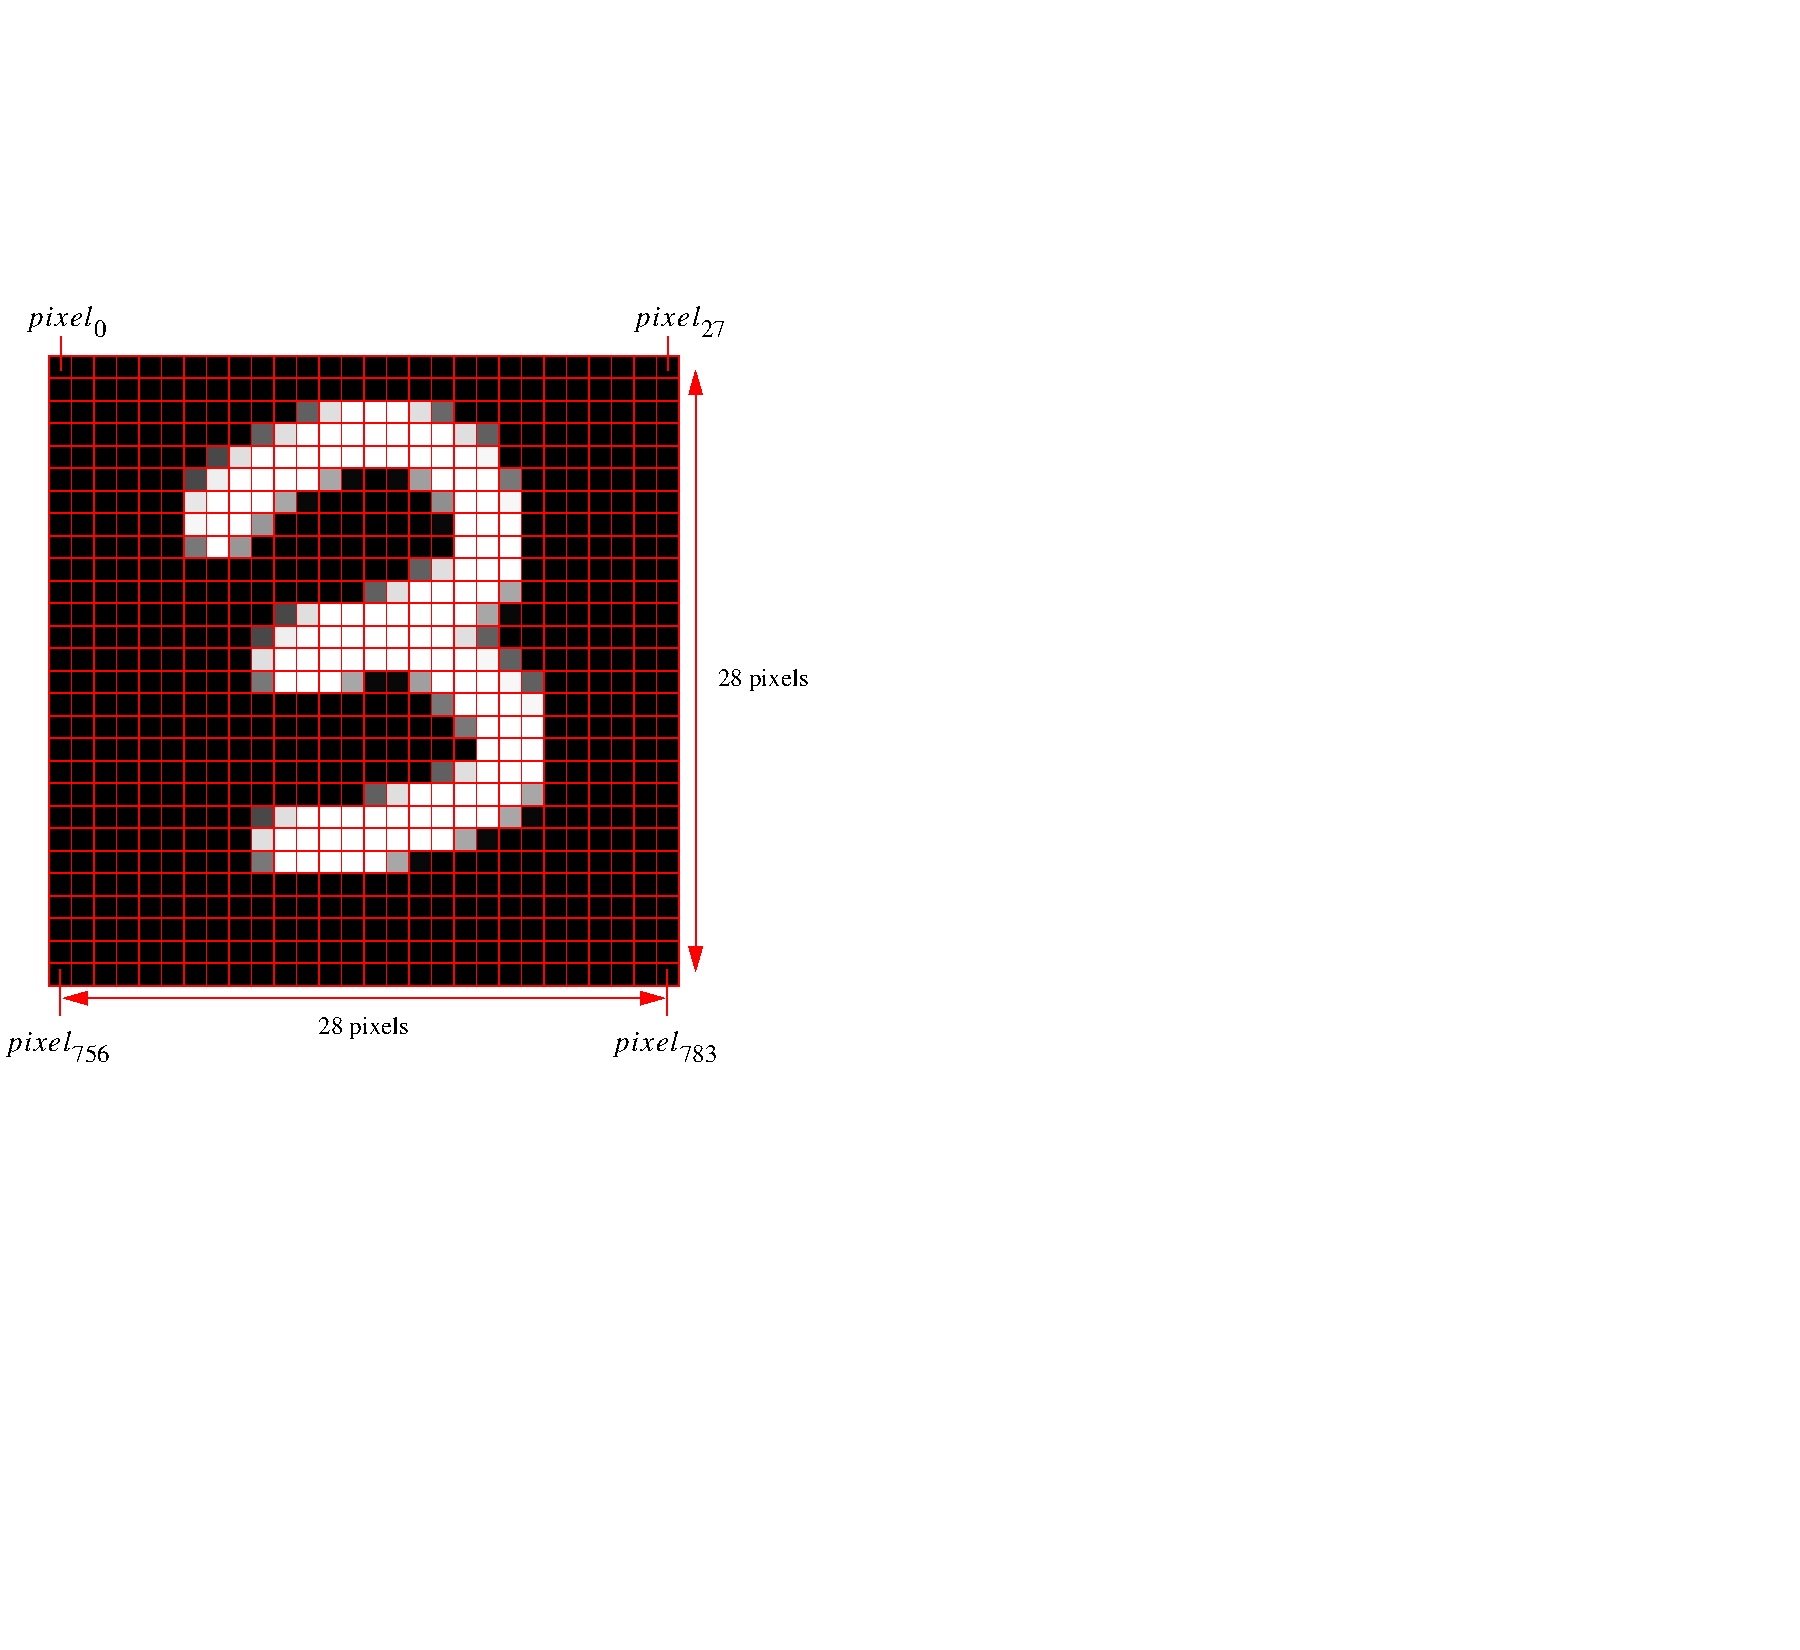
\includegraphics[scale=0.7]{figures/fig_mnist_image}
   \end{center}
   \caption{An example handwritten digit image from the MNIST database}
	\label{fig:mnist_image}
\end{figure}

The database contains a training set of 60000 images which are used to train the classifier, and a test set of 10000 images which are used to test the classifier's accuracy. 
The 60000 training images have already been used to train the weights for the classifier. 
Your task is to use the provided weights to implement the classifier and test its classification accuracy on the 10000 test images.

\section*{A Simple CNN-Based Classifier for MNIST Digits}

\begin{figure}[H]
   \begin{center}
       \hspace*{0.1cm}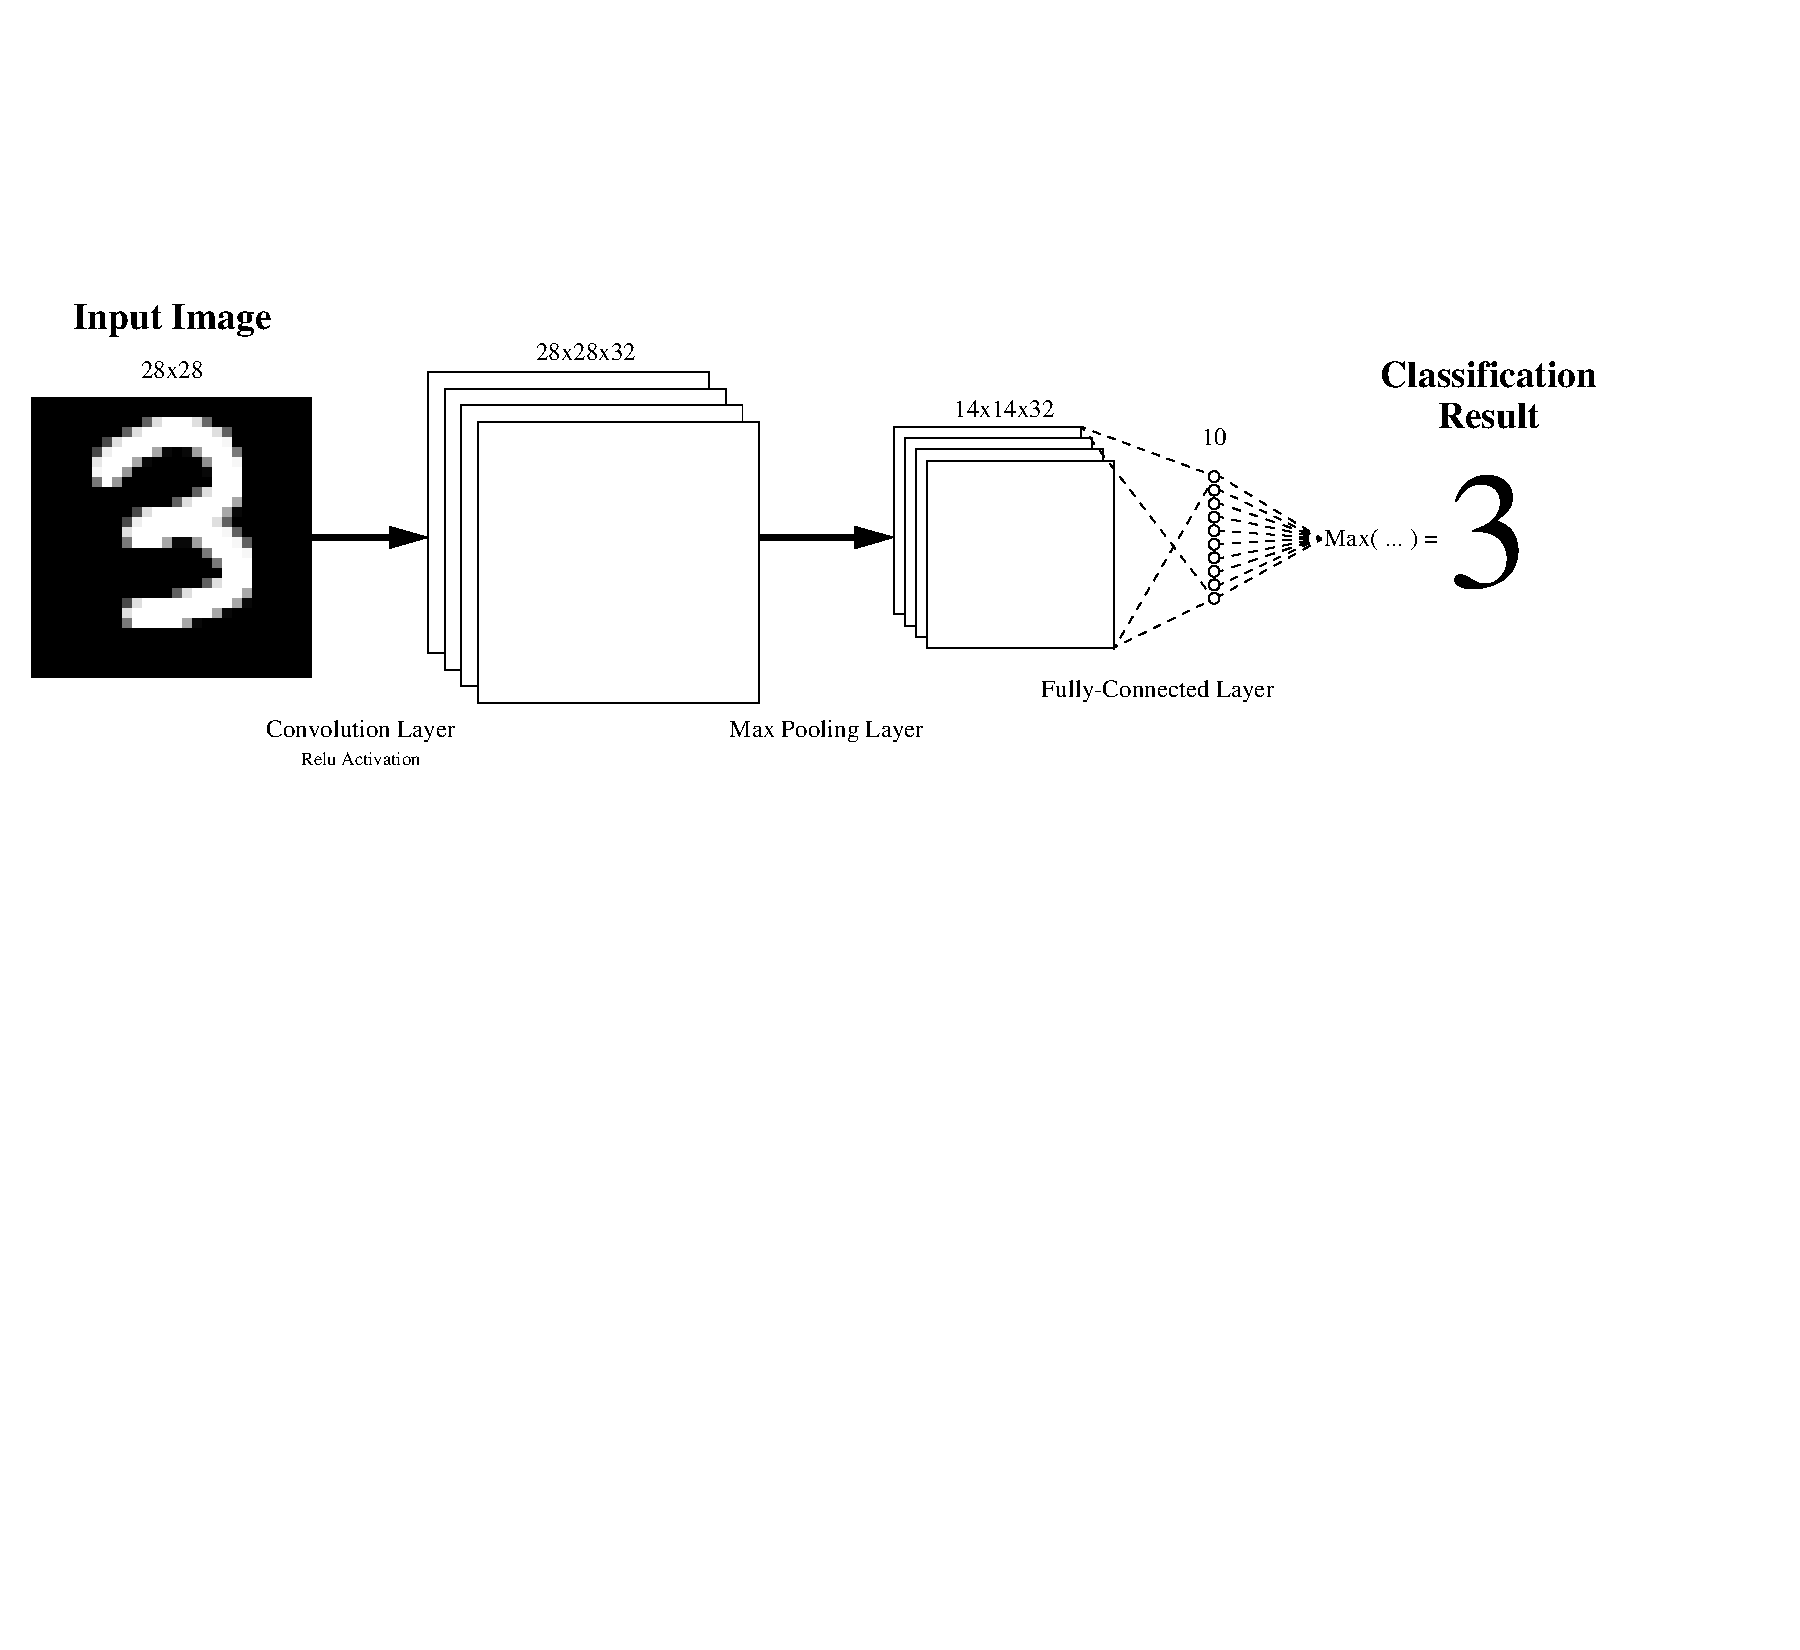
\includegraphics[scale=0.6]{figures/fig_cnn_classifier}
   \end{center}
   \caption{The layers of the CNN-based classifier}
	\label{fig:cnn_classifier}
\end{figure}

You will implement the CNN-based Classifier shown in Figure~\ref{fig:cnn_classifier}. 
The classifier accepts an MNIST digit image as input which has the dimensions 28x28. 
The classifier provides as output the classification result, ranging 0 to 9.  
Between the input and output layers, the classifier contains three hidden layers which are described in the following sections.

\subsection*{The Convolution Layer}

\begin{figure}[H]
   \begin{center}
       \hspace*{0.1cm}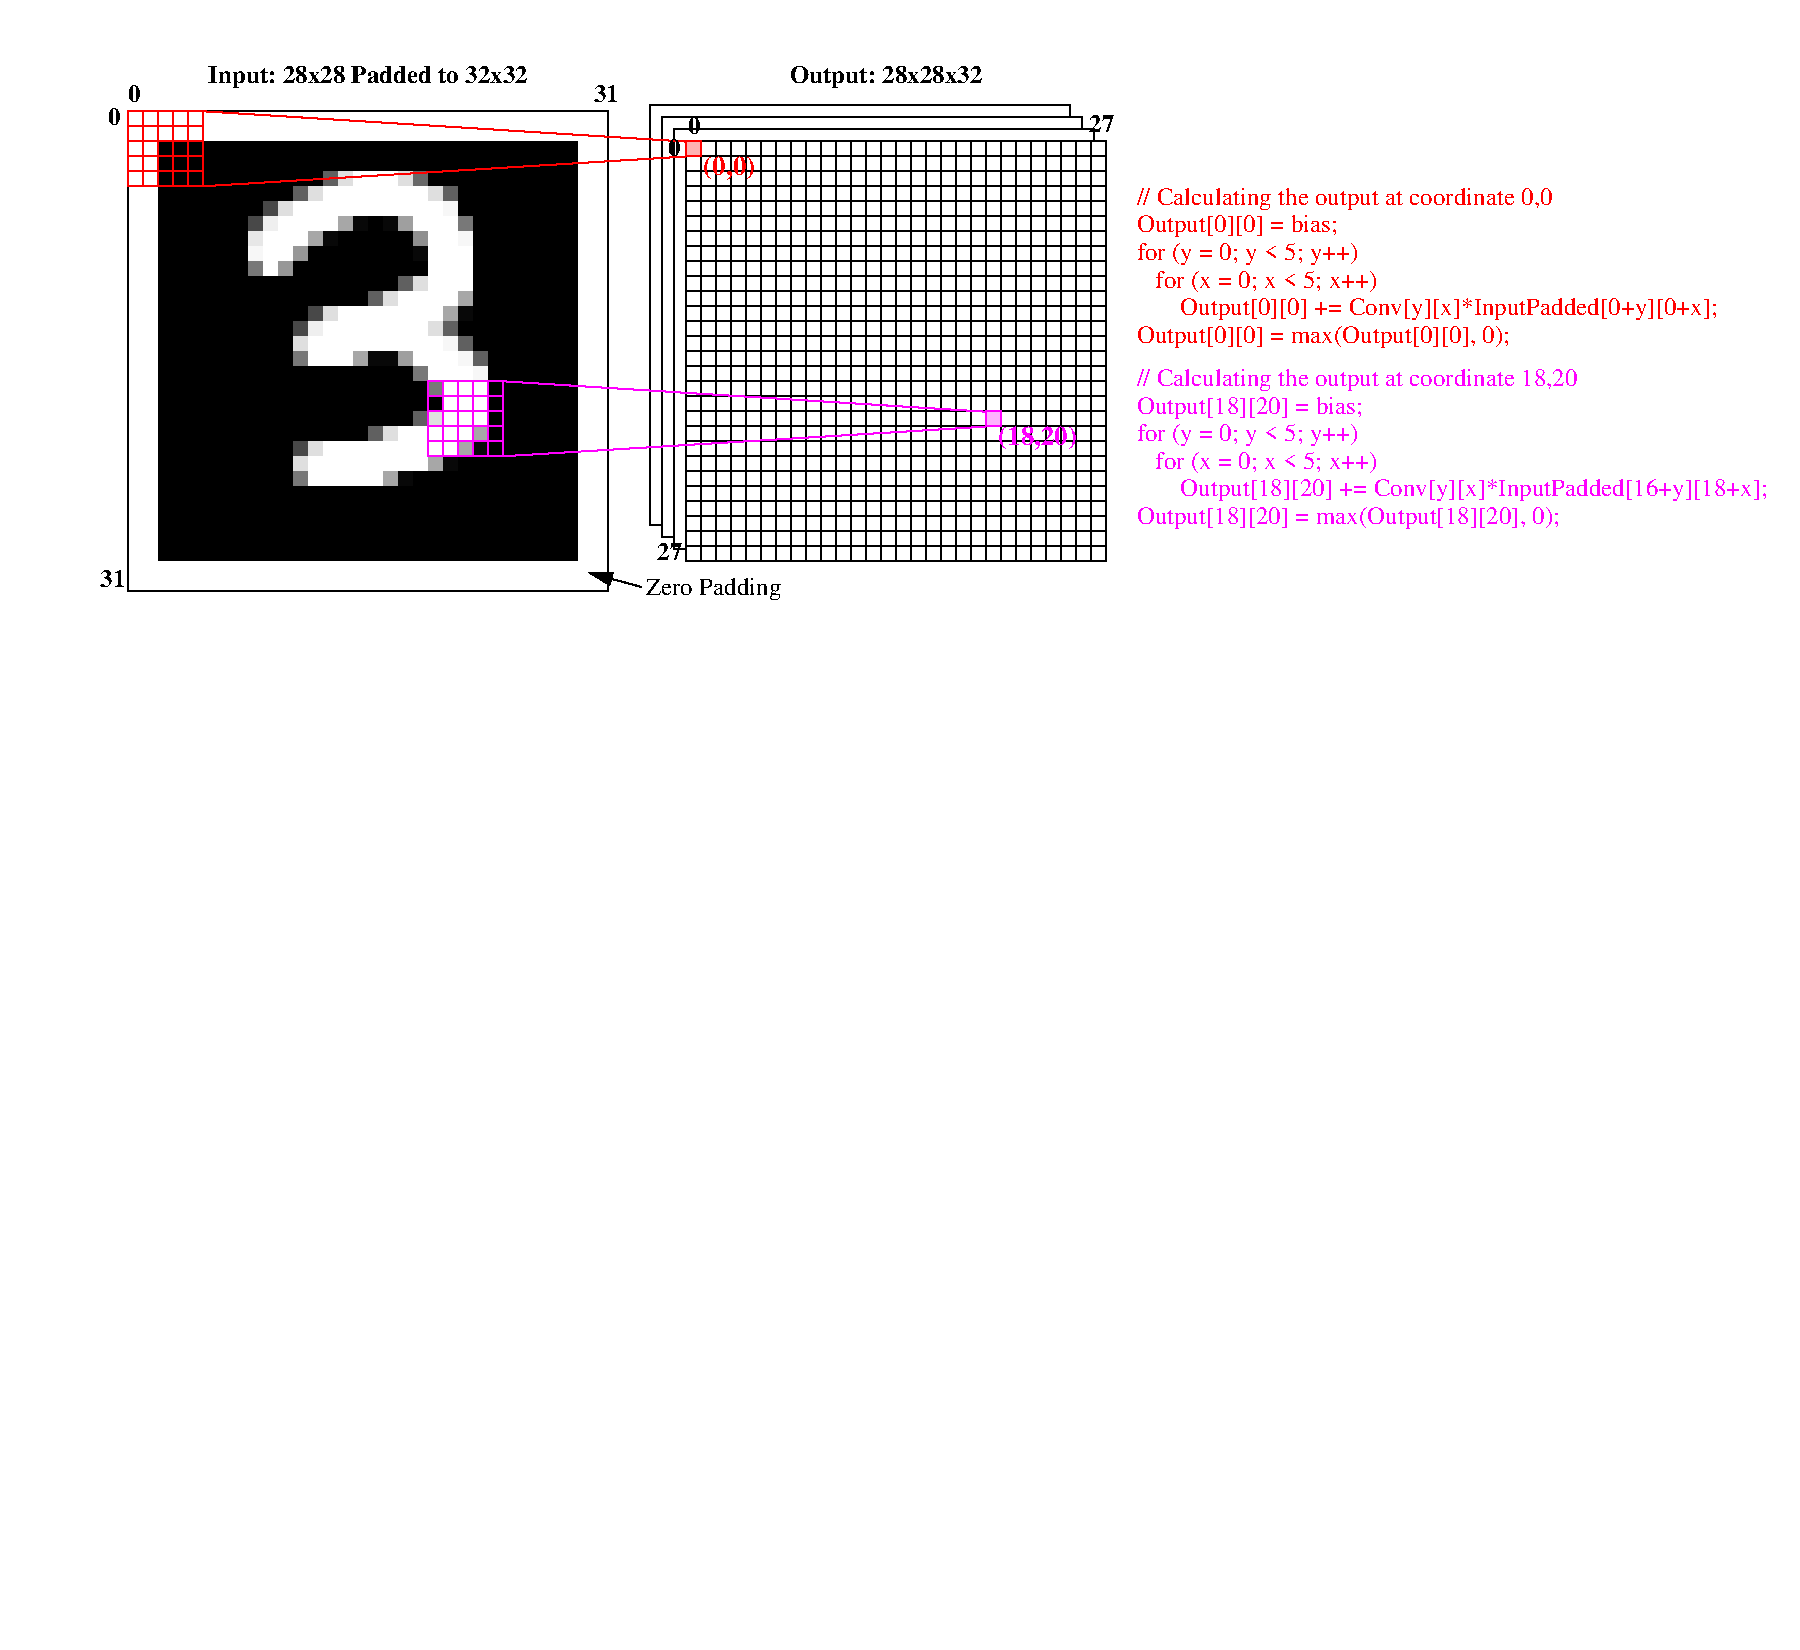
\includegraphics[scale=0.6]{figures/fig_cnn_layer}
   \end{center}
   \caption{Applying a convolutional matrix to the input image with calculations shown for two of the output values}
	\label{fig:cnn_layer}
\end{figure}

The convolution layer applies 32 5x5 convolutional matrices on the input image to yield 32 feature maps. 
Before convolving, the layer adds 2-pixel zero padding to all edges of the input image so that the output map retains the same dimensions as the input image.
Each convolutional matrix is applied to 5x5 patches of the padded image using a stride of 1 pixel.
Each convolutional matrix has an associated trained bias value which is added to each convolution result.
The ReLU activation function (defined as ReLU(x) = x > 0 ? x : 0) is then applied to the biased convolution result.
The ReLU-activated value is then written to the output feature map.
Figure~\ref{fig:cnn_layer} shows a convolutional matrix being applied to the input image to yield one feature map.
The figure shows the calculations involved in producing two of the values in the output feature map.
In the end, the 32 convolutional matrices yield 32 28x28 feature maps for a total output with dimensions 28x28x32. 

\subsection*{The Max Pooling Layer}

\begin{figure}[H]
   \begin{center}
       \hspace*{0.1cm}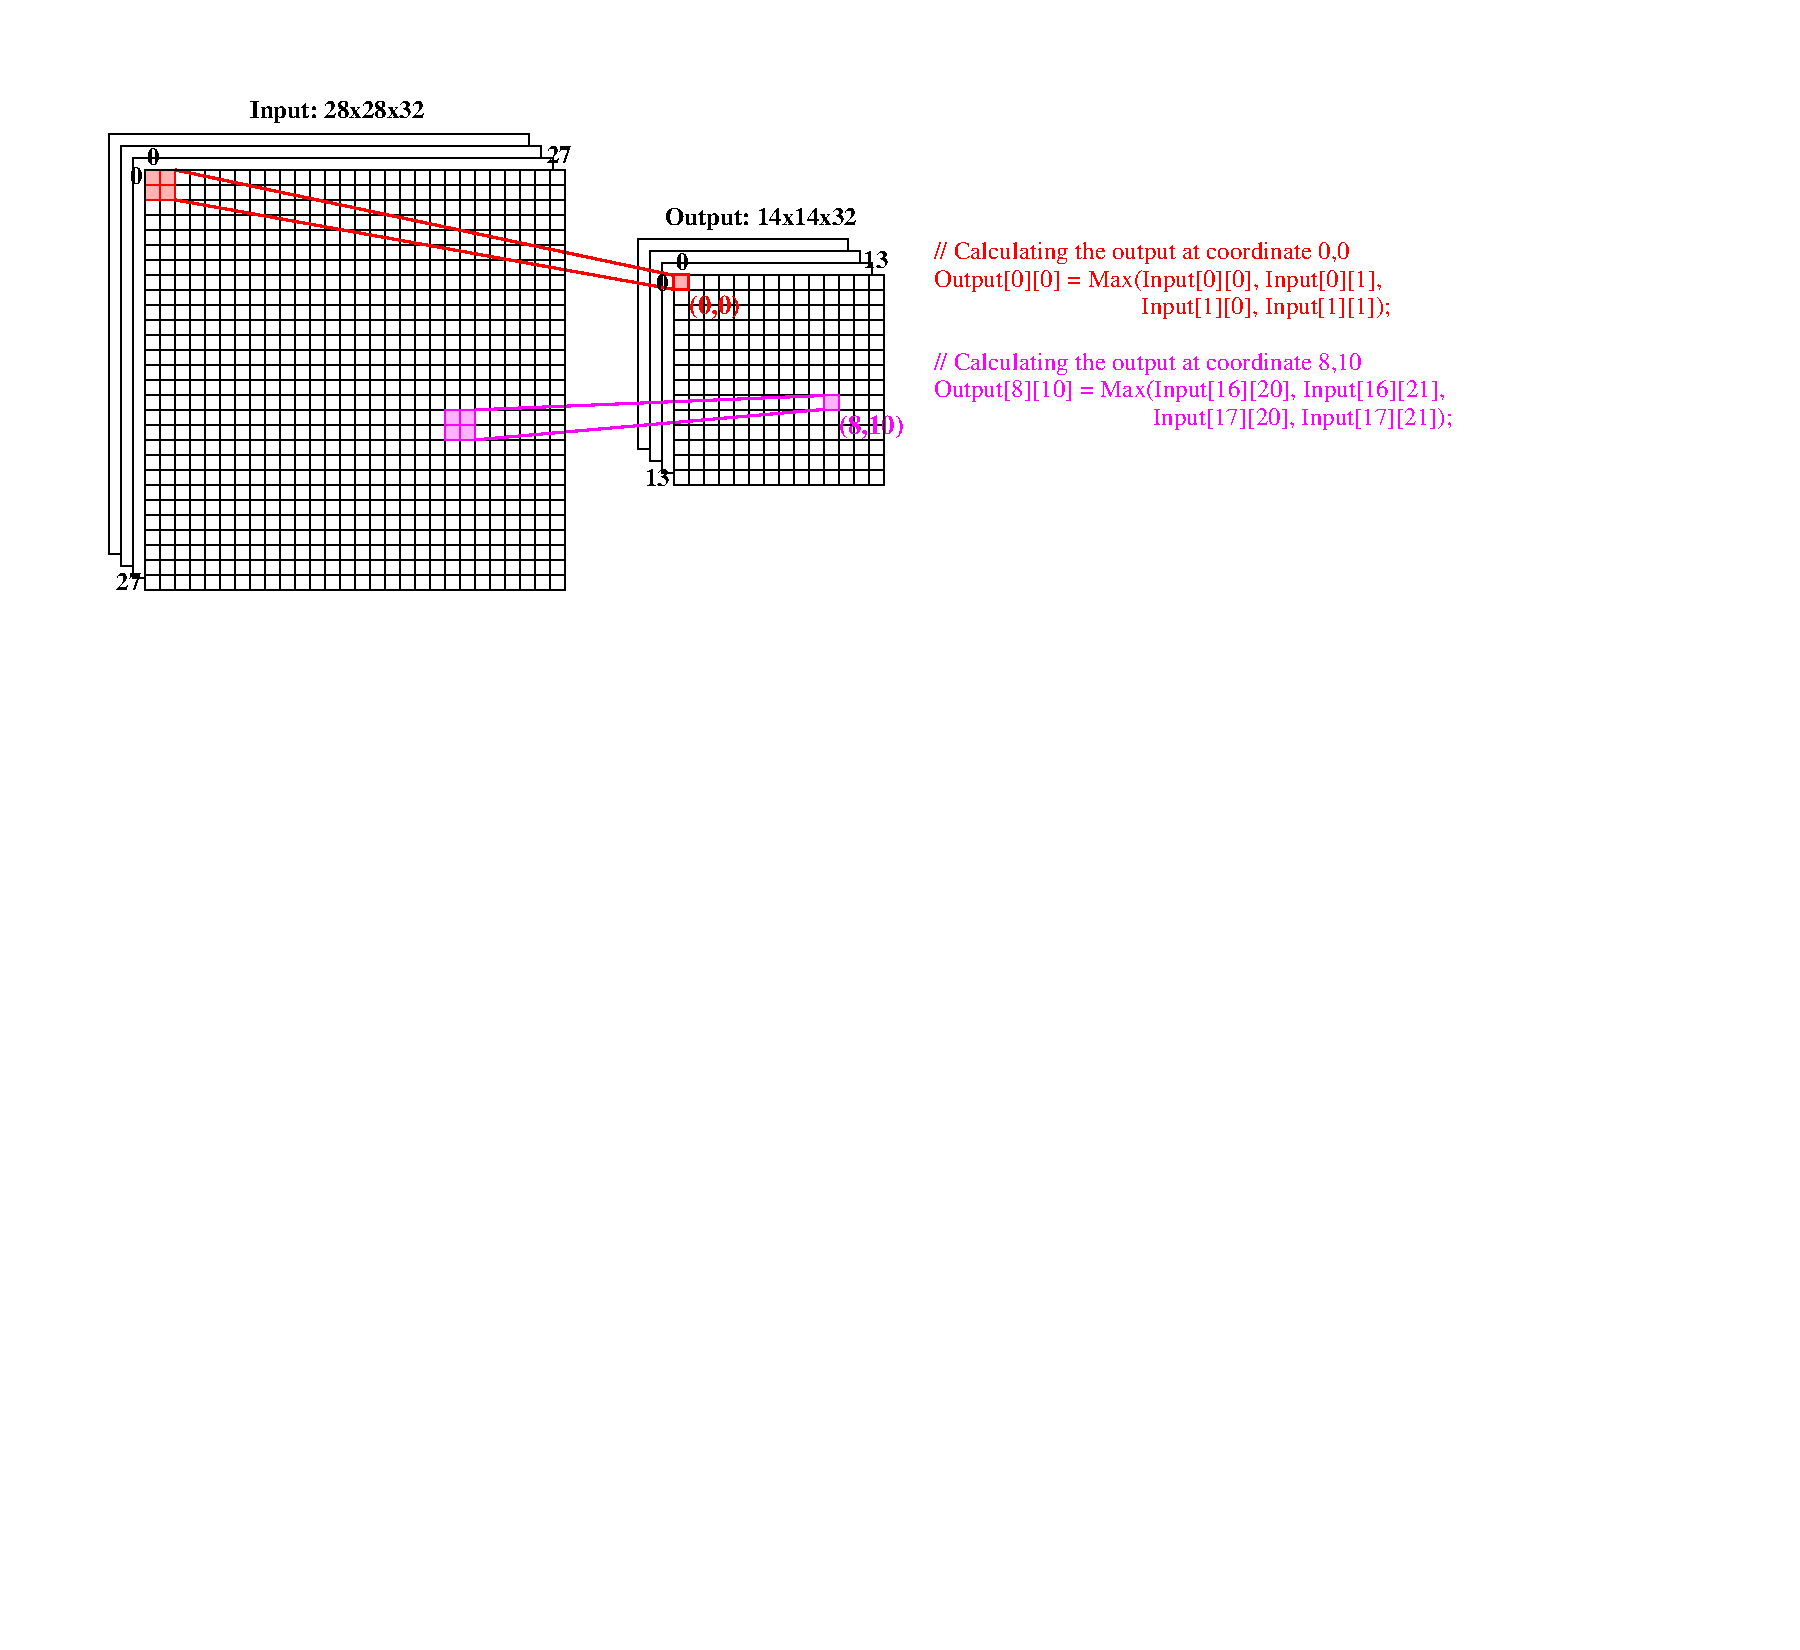
\includegraphics[scale=0.7]{figures/fig_pooling_layer}
   \end{center}
   \caption{Applying the 2x2 max pooling on a 28x28 input with calculations shown for two of the output values}
	\label{fig:pooling_layer}
\end{figure}

The max pooling layer downsamples the feature maps produced by the CNN layer by retaining only the maximum value in each 2x2 block
of values. Downsampling in this layer reduces the number of features in flight  and thus the number of calculations required in the subsequent layers.
It also reduces the amount of memory required to store subsequent  features.
By applying 2x2 max pooling with a stride of 2 pixels on a 28x28x32 input, the layer produces an output with dimensions 14x14x32. 

\subsection*{The Fully Connected Layer}

\begin{figure}[H]
   \begin{center}
       \hspace*{0.1cm}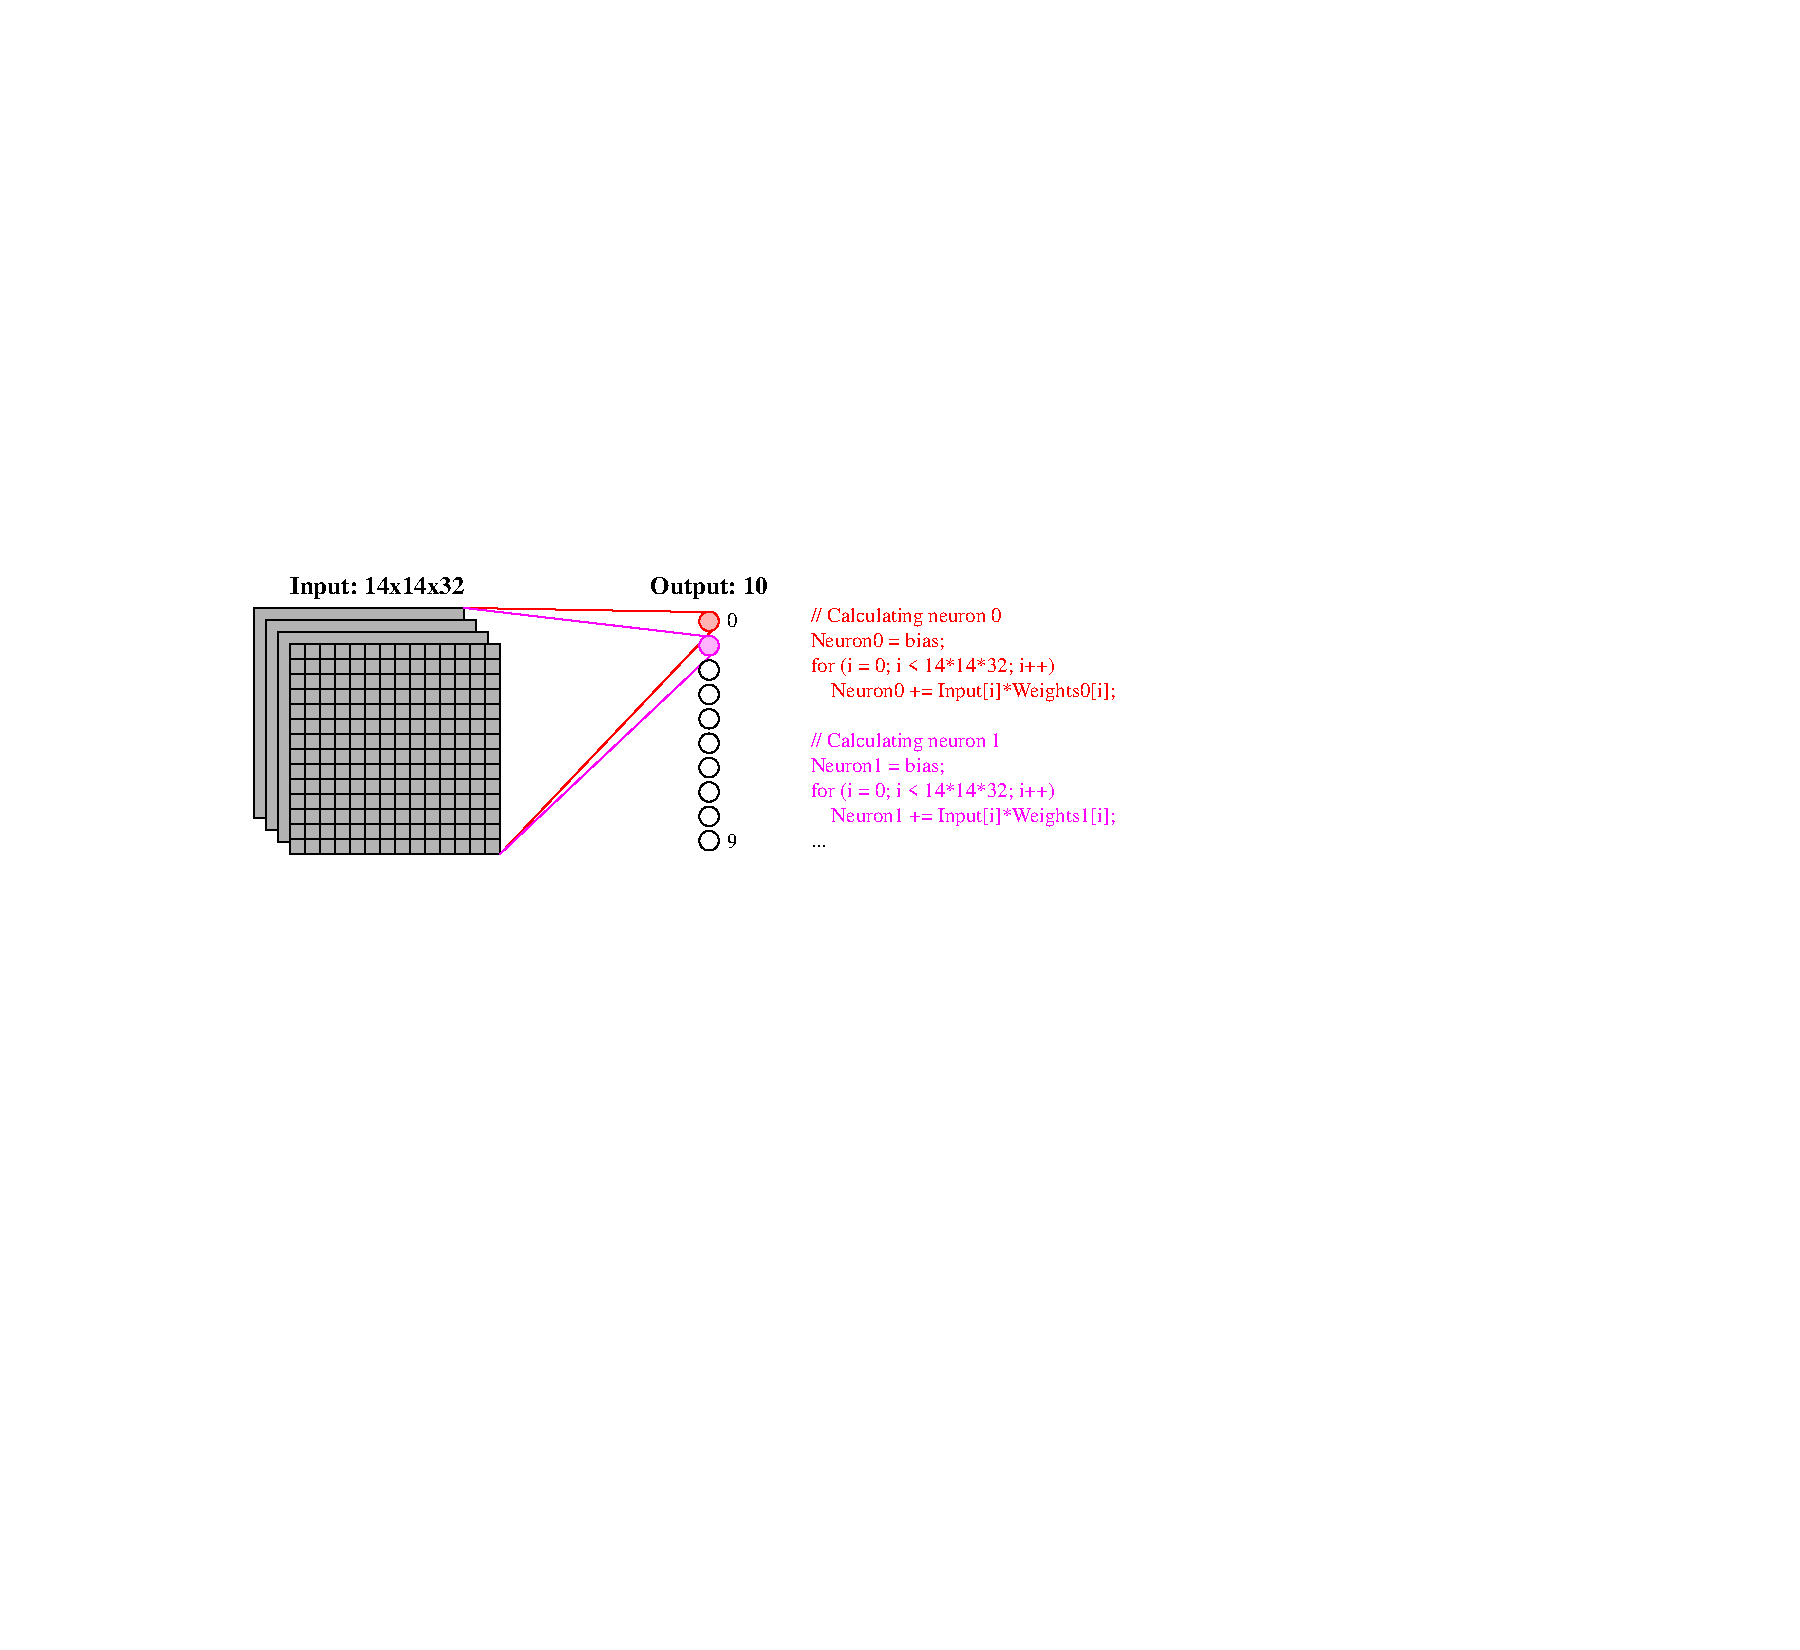
\includegraphics[scale=1.0]{figures/fig_fc_layer}
   \end{center}
   \caption{The fully connected layer with calculations shown for two of the output neurons}
	\label{fig:fc_layer}
\end{figure}

The fully connected layer yields 10 output neurons, each of which is calculated as the weighted sum of the 14x14x32 features output from the
previous layer. This means that in total there are 14x14x32x10 = 62720 weights.  
In essence, this fully-connected layer is a linear classifier whose input are the features outputted by the max pooling layer,
and output are the likelihoods of the input image belonging to each of the 10 digit classes.
The digit with the highest output value is chosen as the classification result.

\section*{Part I}
\noindent
Implement a program in the C++ language that performs CNN-based classification of MNIST handwritten digits as described in the previous section.
Use the trained weights provided in the \textit{/design\_files/weights\_fxp/} directory. 
Test your program by classifying the 10000 MNIST test images stored in the file \textit{/design\_files/t10k-images-idx3-ubyte}. 
Compare the results of your classifier to the correct labels stored in the file \textit{/design\_files/t10k-labels-idx1-ubyte} to calculate
your classifier's accuracy as: \[Accuracy = (\#\ of\ correct\ results )/ 10000 * 100\% \]
Compile and execute your program on a DE-Series Linux platform.
Upon completion, your program should output the classification accuracy and the runtime in milliseconds.

\subsubsection*{Parsing the MNIST Database Files}
The MNIST database is provided in .idx files. The file formats of the MNIST images and labels files are shown in Figure~\ref{fig:mnist_file_format}. 
Your program must open and parse these files to extract the image pixels and labels. Each pixel is 8 bits and represents a grayscale value.
Each label is also 8 bits, and its value can range from 0 to 9 to indicate the correct classification of the corresponding image.
The 32-bit integers stored in these files are stored in most-significant byte (MSB)-first format, which
must first be converted to least significant byte (LSB)-first format before being used on the ARM processors of the DE-series boards.

\lstset{}
\begin{figure}[H]
\begin{center}
\begin{minipage}[t]{12.7 cm}
\begin{lstlisting}
TEST SET IMAGE FILE (t10k-images-idx3-ubyte):
[offset] [type]          [value]          [description] 
0000     32 bit integer  0x00000803(2051) magic number 
0004     32 bit integer  10000            number of images 
0008     32 bit integer  28               number of rows 
0012     32 bit integer  28               number of columns 
0016     unsigned byte   ??               pixel 
0017     unsigned byte   ??               pixel 
........ 
xxxx     unsigned byte   ??               pixel

TEST SET LABEL FILE (t10k-labels-idx1-ubyte):
[offset] [type]          [value]          [description] 
0000     32 bit integer  0x00000801(2049) magic number (MSB first) 
0004     32 bit integer  10000            number of items 
0008     unsigned byte   ??               label 
0009     unsigned byte   ??               label 
........ 
xxxx     unsigned byte   ??               label
The labels values are 0 to 9.
\end{lstlisting}
\end{minipage}
\end{center}
\vspace{-.23in}\caption{File formats of the MNIST files. Source: http://yann.lecun.com/exdb/mnist/}
\label{fig:mnist_file_format}
\end{figure}

\subsubsection*{Parsing the Weights Files}

Trained neural network weights are provided in the directory \textit{/design\_files/weights\_fxp/}. The weights are in 16-bit (8.8) fixed-point format.
In the directory are 10 files named 
\textit{fc\_weights\_0}, \textit{fc\_weights\_1}, ... , \textit{fc\_weights\_9} that provide the weights for the 10 neurons of the fully-connected layer.
%Each of these files provides the weights for one of the digits from 0 to 9 as suffixed to the file names.
The digit for which the file provides the weights is suffixed to the file name.
The weights in these files are arranged row-first, starting with weight corresponding to coordinate 0,0 (top-left) of feature map 0 (the output map of convolutional matrix 0). 
Finally there is one weights file named \textit{cnn\_weights} which provide the weights for the 32 5x5 convolutional matrices of the CNN layer.
The \textit{cnn\_weights} file contains 32 sets of 26 weights, where the first 25 of each set of 26 correspond to the 5x5 matrix weights, and the 26th 
is the bias. The file stores the sets starting from convolutional matrix 0. The 5x5 matrix weights are arranged row-first starting from coordinate 0,0 (top-left) of the 5x5 matrix. 
The files can be parsed using the code shown in Figure~\ref{fig:parse_weights_code}. 

\lstset{language=C++}
\begin{figure}[H]
\begin{center}
\begin{minipage}[t]{16 cm}
\begin{lstlisting}
// weights must be an array of sufficient size (>= num_weights)
bool read_weights_file(char *filename, short *weights, int num_weights) {
	FILE *f = fopen(filename, "rb");
	if (f == NULL){
		printf("ERROR: could not open %s\n",filename);
		return false;
	}
	int read_elements = fread(weights, sizeof(short), num_weights, f);
	fclose(f);
	
	if (read_elements != num_weights){
		printf("ERROR: read incorrect number of weights from %s\n", filename);
		return false;
	}
	return true;
}
\end{lstlisting}
\end{minipage}
\end{center}
\vspace{-0.33in}\caption{Function that parses a weights file}
\label{fig:parse_weights_code}
\end{figure}

\section*{Part II}

Create an OpenCL implementation of the CNN-based classifier you created in Part I. You may wish to reuse code from your linear classifier in Exercise 4 to implement the fully-connected layer. Consider whether you will implement a single monolithic OpenCL kernel or divide the work into multiple smaller kernels. If implementing multiple kernels, decide whether to use global memory or pipes to share the data. Carefully consider how you will utilize the limited local memory resources to maximize performance.
Finally, output the accuracy and runtime of your implementation and compare them to your results in Part I.

\section*{Part III (Bonus)}

Devise a neural network topology for a classifier that improves on the accuracy you achieved in Part II. 
Create an OpenCL implementation of your classifier. As you will be limited by the amount of resources available to you, 
carefully consider the tradeoffs between accuracy, runtime, and FPGA resource usage. 
The parameters that you can adjust include:

\begin{itemize}
\item Number of CNN layers, convolutional matrix size(s), number of matrices per layer, stride size
\item Number of pooling layers, size, and stride
\item Number of FC layers, and number of intermediate neurons
\item Precision (8, 16, 32 bit fixed-point, decimal position, mixed precision)
\end{itemize}

To train weights you can use a machine learning framework of your choice. Some common frameworks include Tensorflow and Caffe. 

%%%%%%%%%%%%%%%%%%%%%%%%%%%%%%%%%%%%%%%%
%%% FPGAcademy Copyright Information %%%
%%%%%%%%%%%%%%%%%%%%%%%%%%%%%%%%%%%%%%%%

%Always put the copyright on a new page (clear page), with some vertical space from top
\clearpage
\vspace{1in}

\noindent

Copyright {\copyright} FPGAcademy.org. All rights reserved. FPGAcademy and the 
FPGAcademy logo are trademarks of FPGAcademy.org.  This document is provided 
"as is", without warranty of any kind, express or implied, including but not 
limited to the warranties of merchantability, fitness for a particular purpose 
and noninfringement. In no event shall the authors or copyright holders be 
liable for any claim, damages or other liability, whether in an action of 
contract, tort or otherwise, arising from, out of or in connection with the 
document or the use or other dealings in the document.
~\\
~\\
**Other names and brands may be claimed as the property of others.


\end{document}
